\pdfoutput=1 % only if pdf/png/jpg images are used
\documentclass{JINST}

\usepackage{amsmath,amssymb}
\usepackage[numbers,sort]{natbib}
%\hypersetup{colorlinks, citecolor=blue, linkcolor=blue, filecolor=blue, urlcolor=red}

\title{Background rejection in NEXT using deep neural networks}

\author{Author 1$^a$\thanks{Corresponding author.},
Author 2$^b$\\
\llap{$^a$}Instituto de F\'isica Corpuscular (IFIC), CSIC \& Universitat de Val\`encia,\\ 
Calle Catedr\'atico Jos\'e Beltr\'an, 2, 46980 Paterna, Valencia, Spain\\
\llap{$^b$}University of Texas at Arlington\\
 701 S. Nedderman Drive, Arlington, TX 76019, USA\\
E-mail: \email{correspodingauthor@ific.uv.es}\\

NEXT Collaboration}

\bibliographystyle{unsrtnat}
%%%%%%%%%%%%%%%%%%%%%%%%%%%%%%%%%%%%%%%%%%%%%%%%%%
% $Id: commands.tex 1931 2015-01-17 10:32:50Z jmalbos $
% Some useful new commands...

%%%%%%%%%%%%%%%%%%%%%%%%%%%%%%%%%%%%%%%%%%%%%%%%%%
% BB
\newcommand{\bb}{\ensuremath{\beta\beta}}
% BB0NU
\newcommand{\bbonu}{\ensuremath{0\nu\beta\beta}}
% BB2NU
\newcommand{\bbtnu}{\ensuremath{2\nu\beta\beta}}

%%%%%%%%%%%%%%%%%%%%%%%%%%%%%%%%%%%%%%%%%%%%%%%%%%
% mBB
\newcommand{\mbb}{\ensuremath{m_{\bb}}}
% T0nu
\newcommand{\Tonu}{\ensuremath{T_{1/2}^{0\nu}}}
% Gonu
\newcommand{\Gonu}{\ensuremath{G^{0\nu}}}
% MNE
\newcommand{\Monu}{\ensuremath{\left|M^{0\nu}\right|}}
% Qbb
\newcommand{\Qbb}{\ensuremath{Q_{\bb}}}

%%%%%%%%%%%%%%%%%%%%%%%%%%%%%%%%%%%%%%%%%%%%%%%%%%
% kg·year
\newcommand{\kgy}{\ensuremath{\mathrm{kg}\cdot\mathrm{yr}}}
% Mbb
\newcommand{\Mbb}{\ensuremath{M_{\bb}}}
% kgbb
\newcommand{\kgbb}{\ensuremath{\mathrm{kg}_{\bb}}}
% ckky
\newcommand{\ckky}{\ensuremath{\mathrm{cts~keV^{-1}~kg^{-1}~yr^{-1}}}}
% ckkbby TO BE REVISED
\newcommand{\ckkbby}{\ckky}

%%%%%%%%%%%%%%%%%%%%%%%%%%%%%%%%%%%%%%%%%%%%%%%%%%
% Ca-48
\newcommand{\CA}{\ensuremath{^{48}\mathrm{Ca}}}
% Ge-76
\newcommand{\GE}{\ensuremath{^{76}\mathrm{Ge}}}
% Se-82
\newcommand{\SE}{\ensuremath{^{82}\mathrm{Se}}}
% Zr-96
\newcommand{\ZR}{\ensuremath{^{96}\mathrm{Zr}}}
% Mo-100
\newcommand{\MO}{\ensuremath{^{100}\mathrm{Mo}}}
% Pd-110
\newcommand{\PD}{\ensuremath{^{110}\mathrm{Pd}}}
% Cd-116
\newcommand{\CD}{\ensuremath{^{116}\mathrm{Cd}}}
% Sn-124
\newcommand{\SN}{\ensuremath{^{124}\mathrm{Sn}}}
% Te-130
\newcommand{\TE}{\ensuremath{^{130}\mathrm{Te}}}
% Xe-136
\newcommand{\XE}{\ensuremath{^{136}\mathrm{Xe}}}
% Nd-150
\newcommand{\ND}{\ensuremath{^{150}\mathrm{Nd}}}

% Ba-136
\newcommand{\BA}{\ensuremath{^{136}\mathrm{Ba}}}

% Tl-208
\newcommand{\TL}{\ensuremath{^{208}\mathrm{Tl}}}
% Bi-214
\newcommand{\BI}{\ensuremath{^{214}\mathrm{Bi}}}

\newcommand{\URANIUM}{Uranium}
\newcommand{\THORIUM}{Thorium}

% Xe-136
\newcommand{\NA}{\ensuremath{^{22}}Na}
\newcommand{\CS}{\ensuremath{^{137}}Cs}
\newcommand{\SEHF}{\ensuremath{\mathrm{SeF}_6}}
\newcommand{\COT}{\ensuremath{\mathrm{CO}_2}}
\newcommand{\CHF}{\ensuremath{\mathrm{CH}_4}}
\newcommand{\CFF}{\ensuremath{\mathrm{CF}_4}}



%%%%%%%%%%%%%%%%%%%%%%%%%%%%%%%%%%%%%%%%%%%%%%%%%%
% W-values
\newcommand{\Wi}{\ensuremath{W_\mathrm{i}}}
\newcommand{\Wsc}{\ensuremath{W_\mathrm{sc}}}




%%%%%%%%%%%%%%%%%%%%%%%%%%%%%%%%%%%%%%%%%%%%%%%%%%


\abstract{We investigate the potential of using deep learning techniques to reject background events in searches
for neutrinoless double-beta decay with high pressure xenon time projection chambers capable of detailed track
reconstruction.  The differences in the topological signatures of background and signal events can be learned
by deep neural networks via training over many thousands of events.  These networks can then be used to classify
further events as signal or background, providing an additional background rejection factor at an acceptable loss of
efficiency.  This method is found to perform substantially better than previous methods developed based on the use of the
same topological signatures and has the potential for further improvement.}

\keywords{Neutrinoless double beta decay; deep neural networks; TPC; high-pressure xenon chambers;  Xenon; NEXT-100 experiment}

\begin{document}

\section{Introduction}\label{sec:intro}
\noindent Neutrinoless double-beta decay ($0\nu\beta\beta$) is a rare nuclear process in which the nuclear charge changes by two units, and the full energy of the decay ($Q_{\beta\beta}$) is 
emitted in the form of two electrons (or positrons).  It is essentially two simultaneous $\beta^{+}$ or $\beta^{-}$ decays in which no neutrinos are emitted.  While two-neutrino double-beta 
decay ($2\nu\beta\beta$), two simultaneous beta decays in which the two neutrinos are present, is a process predicted by the standard model that has been observed in several isotopes, 
$0\nu\beta\beta$ has never been observed, even after over 75 years of experimental effort.  If $0\nu\beta\beta$ does exist, this implies that the neutrino is its own anti-particle, that is, a
a Majorana particle \cite{Schechter_1982}, amongst other important physical implications (see for example \cite{GomezCadenas:2013ue, Cadenas_2012, Avignone_2008}).

The detection of $0\nu\beta\beta$ decay continues to present unique experimental challenges.  For a given isotope, the lifetime of $0\nu\beta\beta$ decay depends on a nuclear matrix element, 
which can be calculated to some uncertainty, and the square of the effective neutrino mass $|m_{\beta\beta}|^2 = |\sum_{i=e,\nu,\tau}U_{ei}^2m_{i}|^2$ which is a combination of the neutrino
masses $m_{i}$ and neutrino mixing matrix elements $U_{ei}$.  The lifetime is relatively shorter for a degenerate neutrino mass hierarchy ($m_1 \sim m_2 \sim m_3$), longer for an inverted 
neutrino mass hierarchy ($m_1 \ll m_2 < m_3$), and longest for a normal mass hierarchy ($m_1 < m_2 \ll m_3$).  Experiments of the current generation contain approximately
100 kg of the candidate isotope and are subject to several tens of counts per year of background events in their region of interest of energy selection near $Q_{\beta\beta}$.  These experiments
will be capable of probing only the parameter space corresponding to the degenerate mass hierarchy, perhaps pushing into the inverted hierarchy.  In order to completely cover the parameter 
space of the inverted mass hierarchy, experiments employing candidate isotope masses at the ton-scale with background rates of several counts per ton-year will be required.  

NEXT (Neutrino Experiment with a Xenon TPC) \cite{Gomez-Cadenas:2014dxa} will search for neutrinoless double-beta decay in the Lab using a Time Projection Chamber (TPC) filled with 100 kg of 
high-pressure xenon gas (HPXe) at 15 bar pressure enriched to 90\% in the candidate isotope $^{136}$Xe.  The detector will operate using electroluminescent readout (see figure \ref{fig.SS}), in which 
ionization electrons are drifted in a region of relatively low electric field to a narrow region of relatively high electric field, in which they are then accelerated to energies high enough to excite but not 
ionize the atoms of the xenon gas.  These excitations give rise to the emission of electroluminescent light which is detected by an energy plane of 60 photomulitplier tubes (PMTs) and a tracking 
plane of about 8000 silicon photomultipliers (SiPMs).  The detected electroluminescent light signal is called (S2), and can be compared in time with the light detected (S1) due to the excitations 
produced during the initial creation of the ionization track to determine the z-coordinate of its production.  The pattern of light observed on the tracking plane, located just behind the narrow 
electroluminescent region, can be used to obtain the x-y location of the ionization electrons producing the corresponding S2.  The result is a 3D image of the ionization track produced within the 
detector.  The amount of S2 light detected by the energy plane gives an accurate measurement of the energy of the event.  Together this information can be used to identify potential 
$0\nu\beta\beta$ events from the various energy depositions produced in the active volume.

\begin{figure}[!htb]
	\centering
	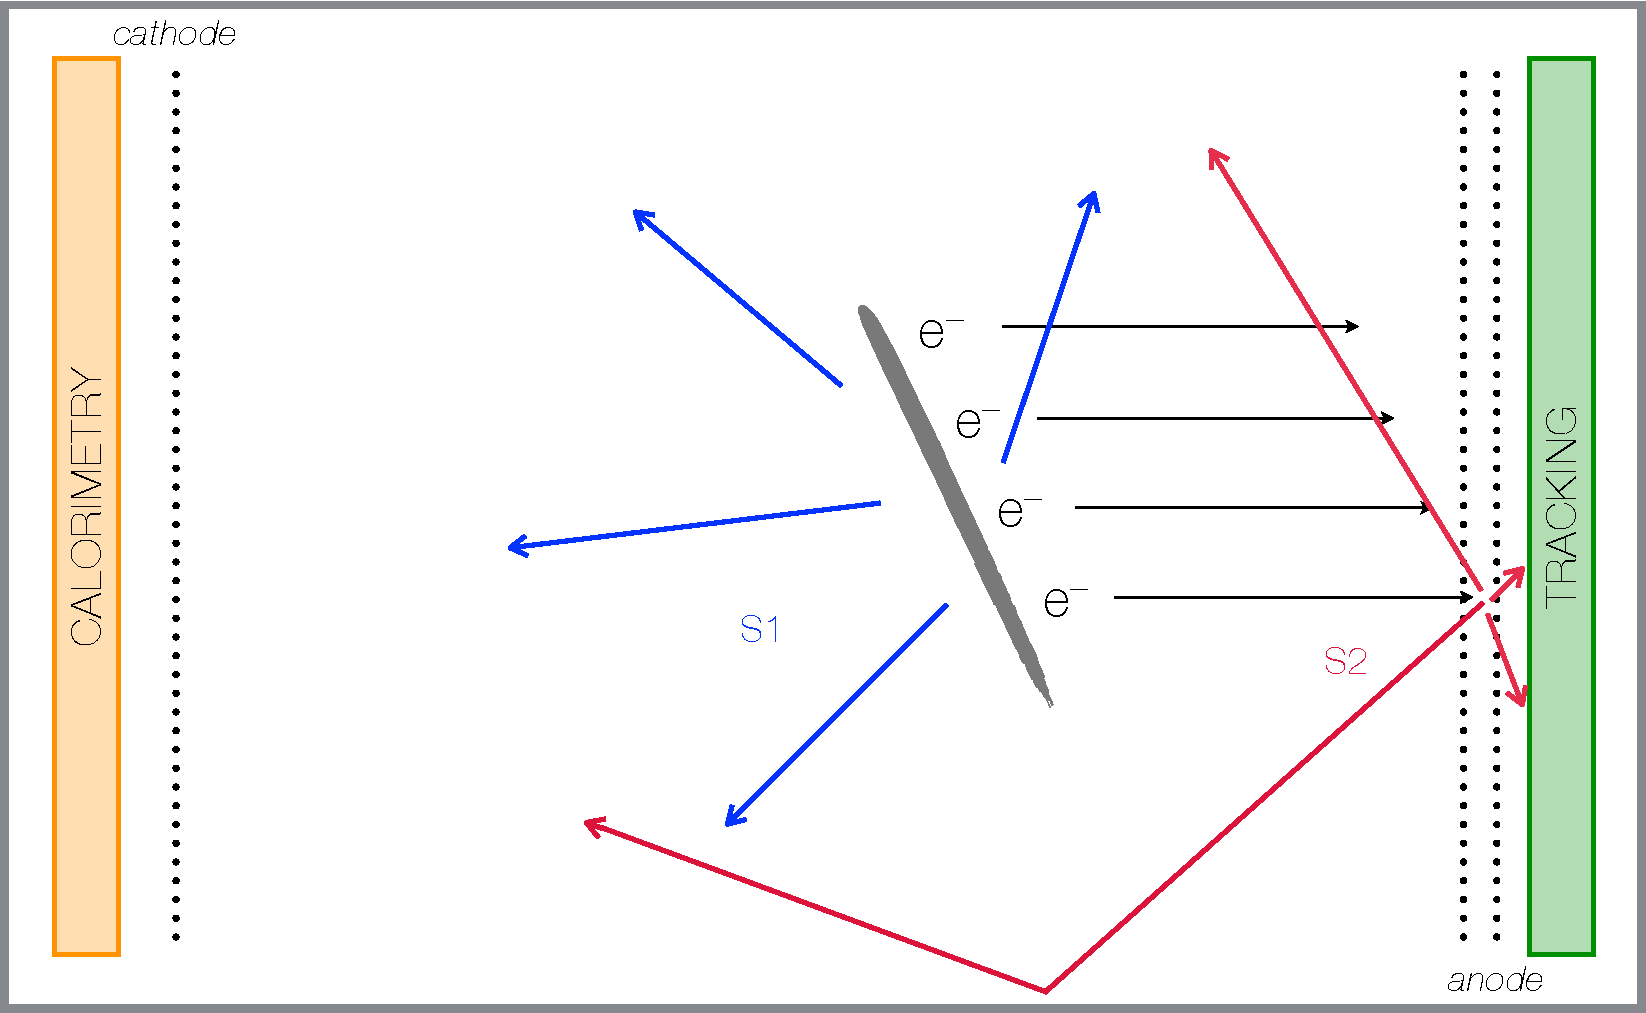
\includegraphics[width= 0.95\textwidth]{fig/SoftAsymmetric_bound.pdf}
	\caption{Production and detection of S1 and S2 in an asymmetric HPXe TPC (figure from \cite{MartinAlbo_thesis}).} \label{fig.SS}
\end{figure}

In addition to performing a competitive search for $0\nu\beta\beta$, NEXT will demonstrate potential 
techniques for operation and background rejection at the ton-scale.  The NEXT collaboration has already built and tested several kg-scale prototypes, NEXT-DBDM \cite{Alvarez:2012kua} and
NEXT-DEMO \cite{Alvarez:2012xda,Alvarez:2012kua,Alvarez:2013gxa,Lorca:2014sra}, which have both demonstrated the excellent energy resolution (extrapolated to 0.5-0.7\% FWHM at
$Q_{\beta\beta}$) obtainable in high pressure xenon gas.  NEXT-DEMO has demonstrated the feasibility of signal/background discrimination based on the topology of reconstructed tracks,
an essential component to identifying $0\nu\beta\beta$ events and rejecting background events (see section \ref{sec:topology}).  The collaboration is currently constructing the first phase of the experiment NEXT-NEW, a 10 kg prototype 
containing about 20\% of the sensors of the 100 kg detector (NEXT-100).  By confirming the ability to obtain good energy resolution and reconstructed tracks at several different scales, NEXT 
intends to confirm the suitability of high pressure xenon gas for operation at the ton-scale.

\section{The NEXT Topological Signature}\label{sec:topology}
One of the most important aspects of NEXT is its ability to image the ionization tracks produced by energetic electrons in its active volume.  Double-beta decay events have a distinct
topological signature produced by two electrons emitted from a common vertex.  Such a track is substantially different from that of a single electron produced, for example, by photoelectric
conversion of a high-energy gamma ray due to several factors.  First, the ionization density ($dE/dx$) increases as energy decreases

%\subsection{Simple Monte Carlo}
%Describe the toy MC (dE/dx, Gaussian MS) and voxelization procedure.
%
%\subsection{GEANT Box Monte Carlo}
%Describe the MAGBOX simulation and Paolina voxelization.
%
%\subsection{NEXT-100 Monte Carlo}
%Describe the NEXT-100 Monte Carlo.  Note that out of the three Monte Carlo simulations discussed, this simulation most closely matches the actual experiment, though it still operates
%directly on Monte Carlo hits and is still not a full simulation with realistic track reconstruction.

\section{Deep Learning}
Short introduction to deep learning

\section{Event classification with a deep neural network (DNN)}
\subsection{Classification procedure}
Describe the data preparation and DNN analysis procedure (input images to Caffe via DIGITS).  Note selection of the GoogLeNet and the use of three 2D projections.

\subsection{Analysis of NEXT-100 Monte Carlo}
Discuss the results obtained with GoogLeNet for NEXT-100 Monte Carlo, to be compared with the topological analysis.  Show the cases of 2x2x2 and 10x10x10 voxels.  This comparison is
the main result of the paper.

\subsection{Evaluating the DNN analysis}
Here we show the DNN analysis for the different Monte Carlo runs, explaining how we arrived at the conclusion that delta rays and energy fluctuations are mainly responsible for the
loss of accuracy.

\section{Conclusions}
DNN analysis with just three projections seems to be capable of outperforming conventional analysis.  Discuss future plans to develop an optimized DNN analysis and speculate
on possible improvements.

%\begin{figure}[!htb]
%\centering
%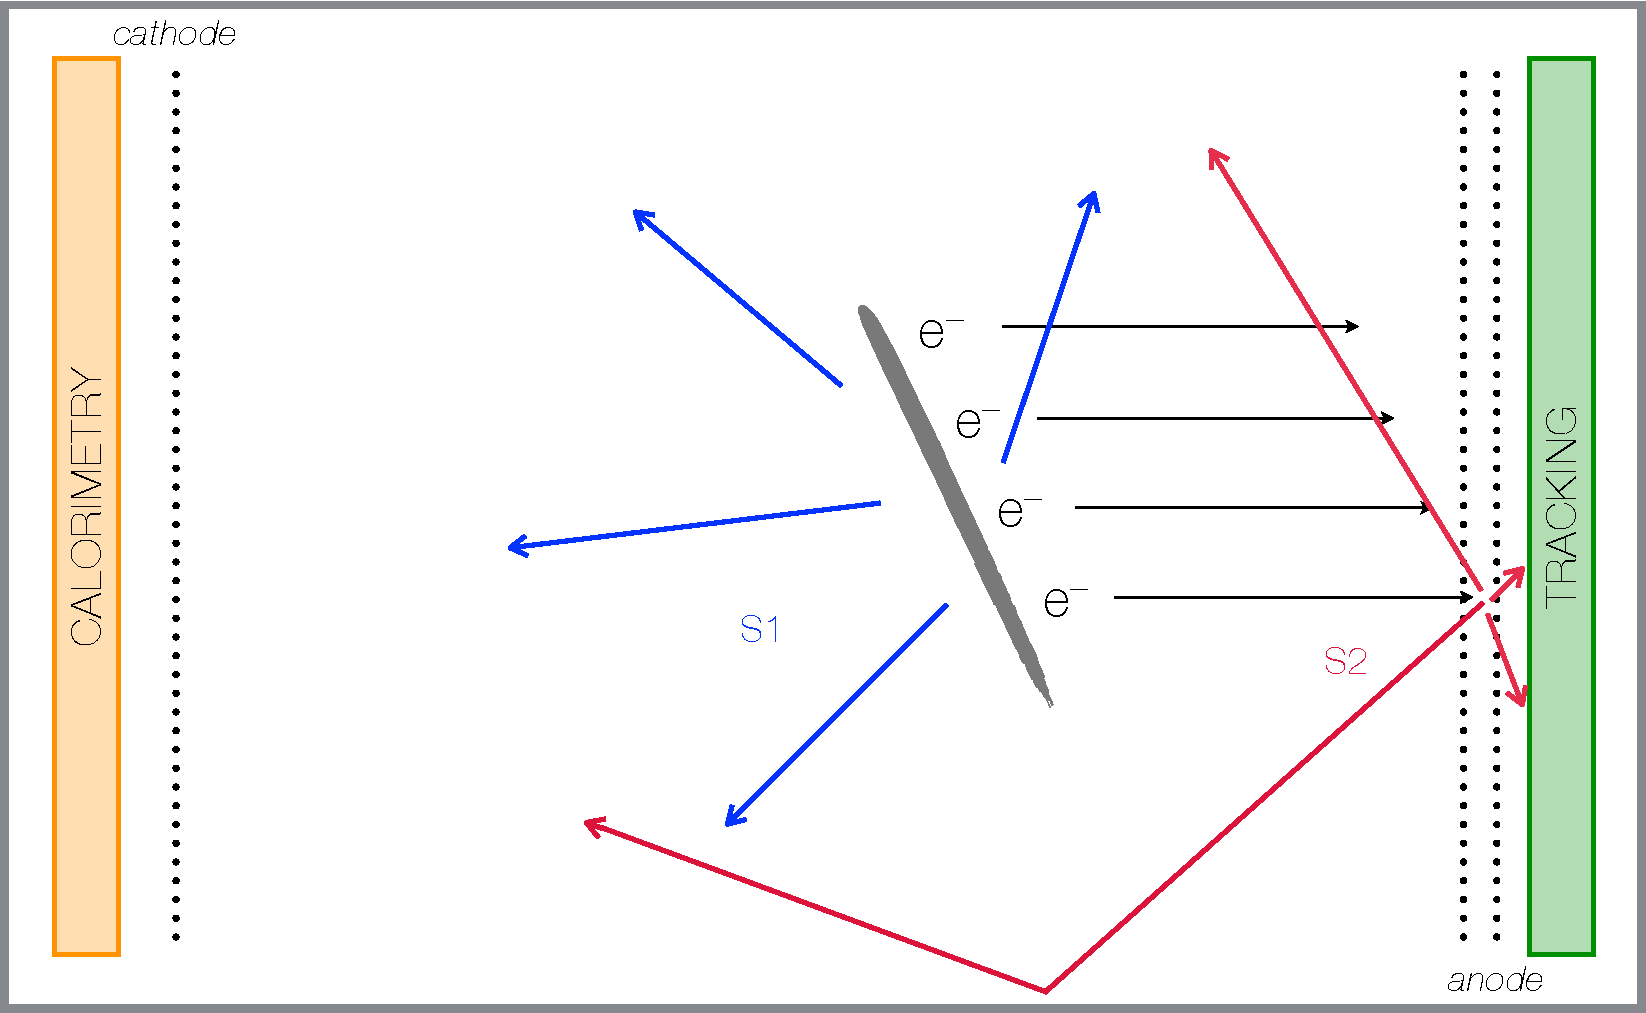
\includegraphics[width= 0.95\textwidth]{fig/SoftAsymmetric_bound.pdf}
%\caption{Principle of operation of an asymmetric HPXe TPC with EL readout (figure from \cite{MartinAlbo_thesis}).} \label{fig.SS}
%\end{figure}

%\appendix
%\section{A Lowpass FIR Filter}\label{app:FIR}

\acknowledgments

This work was supported by the European Research Council under the Advanced Grant 339787-NEXT and the Ministerio de Econom\'{i}a y Competitividad of Spain under Grants CONSOLIDER-Ingenio 2010 CSD2008-0037 (CUP), FPA2009-13697-C04-04, FPA2009-13697-C04-01, FIS2012-37947-C04-01, FIS2012-37947-C04-02, FIS2012-37947-C04-03, and FIS2012-37947-C04-04.  JR acknowledges support from a Fulbright Junior Research Award.

\bibliography{dnnext}


\end{document}